%%http://picat-lang.org/tmp/trace_mapf_grid_sat_2p_0707 : minimize makespan, two-product encoding of amo
%%http://picat-lang.org/tmp/trace_mapf_grid_sat_n2_0707 : minimize makespan, n^2 encoding of amo
%%http://picat-lang.org/tmp/trace_mapf_grid_soc_mip_priorities_basic_0707 : minimize makespan, and soc for the makespan, with priorities using Gurobi
%%http://picat-lang.org/tmp/trace_mapf_grid_soc_sat_0706 : minimize overall soc
%%http://picat-lang.org/tmp/trace_mapf_grid_soc_sat_basic_0706: minimize makespan, and the soc for the makespan
%%http://picat-lang.org/tmp/trace_mapf_grid_soc_sat_priorities_0707 : minimize overall soc with consideration of priorities
%%http://picat-lang.org/tmp/trace_mapf_grid_soc_sat_priorities_basic_0707 : minimize makespan, and then soc for the makespan, with priorities
%% bare_conf.tex
%% V1.4b
%% 2015/08/26
%% by Michael Shell
%% See:
%% http://www.michaelshell.org/
%% for current contact information.
%%
%% This is a skeleton file demonstrating the use of IEEEtran.cls
%% (requires IEEEtran.cls version 1.8b or later) with an IEEE
%% conference paper.
%%
%% Support sites:
%% http://www.michaelshell.org/tex/ieeetran/
%% http://www.ctan.org/pkg/ieeetran
%% and
%% http://www.ieee.org/

%%*************************************************************************
%% Legal Notice:
%% This code is offered as-is without any warranty either expressed or
%% implied; without even the implied warranty of MERCHANTABILITY or
%% FITNESS FOR A PARTICULAR PURPOSE! 
%% User assumes all risk.
%% In no event shall the IEEE or any contributor to this code be liable for
%% any damages or losses, including, but not limited to, incidental,
%% consequential, or any other damages, resulting from the use or misuse
%% of any information contained here.
%%
%% All comments are the opinions of their respective authors and are not
%% necessarily endorsed by the IEEE.
%%
%% This work is distributed under the LaTeX Project Public License (LPPL)
%% ( http://www.latex-project.org/ ) version 1.3, and may be freely used,
%% distributed and modified. A copy of the LPPL, version 1.3, is included
%% in the base LaTeX documentation of all distributions of LaTeX released
%% 2003/12/01 or later.
%% Retain all contribution notices and credits.
%% ** Modified files should be clearly indicated as such, including  **
%% ** renaming them and changing author support contact information. **
%%*************************************************************************


% *** Authors should verify (and, if needed, correct) their LaTeX system  ***
% *** with the testflow diagnostic prior to trusting their LaTeX platform ***
% *** with production work. The IEEE's font choices and paper sizes can   ***
% *** trigger bugs that do not appear when using other class files.       ***                          ***
% The testflow support page is at:
% http://www.michaelshell.org/tex/testflow/



\documentclass[conference]{IEEEtran}
% Some Computer Society conferences also require the compsoc mode option,
% but others use the standard conference format.
%
% If IEEEtran.cls has not been installed into the LaTeX system files,
% manually specify the path to it like:
% \documentclass[conference]{../sty/IEEEtran}





% Some very useful LaTeX packages include:
% (uncomment the ones you want to load)


% *** MISC UTILITY PACKAGES ***
%
%\usepackage{ifpdf}
% Heiko Oberdiek's ifpdf.sty is very useful if you need conditional
% compilation based on whether the output is pdf or dvi.
% usage:
% \ifpdf
%   % pdf code
% \else
%   % dvi code
% \fi
% The latest version of ifpdf.sty can be obtained from:
% http://www.ctan.org/pkg/ifpdf
% Also, note that IEEEtran.cls V1.7 and later provides a builtin
% \ifCLASSINFOpdf conditional that works the same way.
% When switching from latex to pdflatex and vice-versa, the compiler may
% have to be run twice to clear warning/error messages.






% *** CITATION PACKAGES ***
%
%\usepackage{cite}
% cite.sty was written by Donald Arseneau
% V1.6 and later of IEEEtran pre-defines the format of the cite.sty package
% \cite{} output to follow that of the IEEE. Loading the cite package will
% result in citation numbers being automatically sorted and properly
% "compressed/ranged". e.g., [1], [9], [2], [7], [5], [6] without using
% cite.sty will become [1], [2], [5]--[7], [9] using cite.sty. cite.sty's
% \cite will automatically add leading space, if needed. Use cite.sty's
% noadjust option (cite.sty V3.8 and later) if you want to turn this off
% such as if a citation ever needs to be enclosed in parenthesis.
% cite.sty is already installed on most LaTeX systems. Be sure and use
% version 5.0 (2009-03-20) and later if using hyperref.sty.
% The latest version can be obtained at:
% http://www.ctan.org/pkg/cite
% The documentation is contained in the cite.sty file itself.






% *** GRAPHICS RELATED PACKAGES ***
%
\ifCLASSINFOpdf
  % \usepackage[pdftex]{graphicx}
  % declare the path(s) where your graphic files are
  % \graphicspath{{../pdf/}{../jpeg/}}
  % and their extensions so you won't have to specify these with
  % every instance of \includegraphics
  % \DeclareGraphicsExtensions{.pdf,.jpeg,.png}
\else
  % or other class option (dvipsone, dvipdf, if not using dvips). graphicx
  % will default to the driver specified in the system graphics.cfg if no
  % driver is specified.
  % \usepackage[dvips]{graphicx}
  % declare the path(s) where your graphic files are
  % \graphicspath{{../eps/}}
  % and their extensions so you won't have to specify these with
  % every instance of \includegraphics
  % \DeclareGraphicsExtensions{.eps}
\fi
% graphicx was written by David Carlisle and Sebastian Rahtz. It is
% required if you want graphics, photos, etc. graphicx.sty is already
% installed on most LaTeX systems. The latest version and documentation
% can be obtained at: 
% http://www.ctan.org/pkg/graphicx
% Another good source of documentation is "Using Imported Graphics in
% LaTeX2e" by Keith Reckdahl which can be found at:
% http://www.ctan.org/pkg/epslatex
%
% latex, and pdflatex in dvi mode, support graphics in encapsulated
% postscript (.eps) format. pdflatex in pdf mode supports graphics
% in .pdf, .jpeg, .png and .mps (metapost) formats. Users should ensure
% that all non-photo figures use a vector format (.eps, .pdf, .mps) and
% not a bitmapped formats (.jpeg, .png). The IEEE frowns on bitmapped formats
% which can result in "jaggedy"/blurry rendering of lines and letters as
% well as large increases in file sizes.
%
% You can find documentation about the pdfTeX application at:
% http://www.tug.org/applications/pdftex





% *** MATH PACKAGES ***
%
%\usepackage{amsmath}
% A popular package from the American Mathematical Society that provides
% many useful and powerful commands for dealing with mathematics.
%
% Note that the amsmath package sets \interdisplaylinepenalty to 10000
% thus preventing page breaks from occurring within multiline equations. Use:
%\interdisplaylinepenalty=2500
% after loading amsmath to restore such page breaks as IEEEtran.cls normally
% does. amsmath.sty is already installed on most LaTeX systems. The latest
% version and documentation can be obtained at:
% http://www.ctan.org/pkg/amsmath





% *** SPECIALIZED LIST PACKAGES ***
%
%\usepackage{algorithmic}
% algorithmic.sty was written by Peter Williams and Rogerio Brito.
% This package provides an algorithmic environment fo describing algorithms.
% You can use the algorithmic environment in-text or within a figure
% environment to provide for a floating algorithm. Do NOT use the algorithm
% floating environment provided by algorithm.sty (by the same authors) or
% algorithm2e.sty (by Christophe Fiorio) as the IEEE does not use dedicated
% algorithm float types and packages that provide these will not provide
% correct IEEE style captions. The latest version and documentation of
% algorithmic.sty can be obtained at:
% http://www.ctan.org/pkg/algorithms
% Also of interest may be the (relatively newer and more customizable)
% algorithmicx.sty package by Szasz Janos:
% http://www.ctan.org/pkg/algorithmicx




% *** ALIGNMENT PACKAGES ***
%
%\usepackage{array}
% Frank Mittelbach's and David Carlisle's array.sty patches and improves
% the standard LaTeX2e array and tabular environments to provide better
% appearance and additional user controls. As the default LaTeX2e table
% generation code is lacking to the point of almost being broken with
% respect to the quality of the end results, all users are strongly
% advised to use an enhanced (at the very least that provided by array.sty)
% set of table tools. array.sty is already installed on most systems. The
% latest version and documentation can be obtained at:
% http://www.ctan.org/pkg/array


% IEEEtran contains the IEEEeqnarray family of commands that can be used to
% generate multiline equations as well as matrices, tables, etc., of high
% quality.




% *** SUBFIGURE PACKAGES ***
%\ifCLASSOPTIONcompsoc
%  \usepackage[caption=false,font=normalsize,labelfont=sf,textfont=sf]{subfig}
%\else
%  \usepackage[caption=false,font=footnotesize]{subfig}
%\fi
% subfig.sty, written by Steven Douglas Cochran, is the modern replacement
% for subfigure.sty, the latter of which is no longer maintained and is
% incompatible with some LaTeX packages including fixltx2e. However,
% subfig.sty requires and automatically loads Axel Sommerfeldt's caption.sty
% which will override IEEEtran.cls' handling of captions and this will result
% in non-IEEE style figure/table captions. To prevent this problem, be sure
% and invoke subfig.sty's "caption=false" package option (available since
% subfig.sty version 1.3, 2005/06/28) as this is will preserve IEEEtran.cls
% handling of captions.
% Note that the Computer Society format requires a larger sans serif font
% than the serif footnote size font used in traditional IEEE formatting
% and thus the need to invoke different subfig.sty package options depending
% on whether compsoc mode has been enabled.
%
% The latest version and documentation of subfig.sty can be obtained at:
% http://www.ctan.org/pkg/subfig




% *** FLOAT PACKAGES ***
%
%\usepackage{fixltx2e}
% fixltx2e, the successor to the earlier fix2col.sty, was written by
% Frank Mittelbach and David Carlisle. This package corrects a few problems
% in the LaTeX2e kernel, the most notable of which is that in current
% LaTeX2e releases, the ordering of single and double column floats is not
% guaranteed to be preserved. Thus, an unpatched LaTeX2e can allow a
% single column figure to be placed prior to an earlier double column
% figure.
% Be aware that LaTeX2e kernels dated 2015 and later have fixltx2e.sty's
% corrections already built into the system in which case a warning will
% be issued if an attempt is made to load fixltx2e.sty as it is no longer
% needed.
% The latest version and documentation can be found at:
% http://www.ctan.org/pkg/fixltx2e


\usepackage{url,graphicx}
\usepackage{multirow}
\newtheorem{definition}{Definition}
\newcommand{\ignore}[1]{}
%\usepackage{stfloats}
% stfloats.sty was written by Sigitas Tolusis. This package gives LaTeX2e
% the ability to do double column floats at the bottom of the page as well
% as the top. (e.g., "\begin{figure*}[!b]" is not normally possible in
% LaTeX2e). It also provides a command:
%\fnbelowfloat
% to enable the placement of footnotes below bottom floats (the standard
% LaTeX2e kernel puts them above bottom floats). This is an invasive package
% which rewrites many portions of the LaTeX2e float routines. It may not work
% with other packages that modify the LaTeX2e float routines. The latest
% version and documentation can be obtained at:
% http://www.ctan.org/pkg/stfloats
% Do not use the stfloats baselinefloat ability as the IEEE does not allow
% \baselineskip to stretch. Authors submitting work to the IEEE should note
% that the IEEE rarely uses double column equations and that authors should try
% to avoid such use. Do not be tempted to use the cuted.sty or midfloat.sty
% packages (also by Sigitas Tolusis) as the IEEE does not format its papers in
% such ways.
% Do not attempt to use stfloats with fixltx2e as they are incompatible.
% Instead, use Morten Hogholm'a dblfloatfix which combines the features
% of both fixltx2e and stfloats:
%
% \usepackage{dblfloatfix}
% The latest version can be found at:
% http://www.ctan.org/pkg/dblfloatfix




% *** PDF, URL AND HYPERLINK PACKAGES ***
%
%\usepackage{url}
% url.sty was written by Donald Arseneau. It provides better support for
% handling and breaking URLs. url.sty is already installed on most LaTeX
% systems. The latest version and documentation can be obtained at:
% http://www.ctan.org/pkg/url
% Basically, \url{my_url_here}.




% *** Do not adjust lengths that control margins, column widths, etc. ***
% *** Do not use packages that alter fonts (such as pslatex).         ***
% There should be no need to do such things with IEEEtran.cls V1.6 and later.
% (Unless specifically asked to do so by the journal or conference you plan
% to submit to, of course. )


% correct bad hyphenation here
\hyphenation{op-tical net-works semi-conduc-tor}


\begin{document}
%
% paper title
% Titles are generally capitalized except for words such as a, an, and, as,
% at, but, by, for, in, nor, of, on, or, the, to and up, which are usually
% not capitalized unless they are the first or last word of the title.
% Linebreaks \\ can be used within to get better formatting as desired.
% Do not put math or special symbols in the title.
\title{Modeling and Solving the Multi-Agent Pathfinding Problem in Picat}


% author names and affiliations
% use a multiple column layout for up to three different
% affiliations
%\author{\IEEEauthorblockN{Neng-Fa Zhou}
%  \IEEEauthorblockA{CUNY Brooklyn College and Graduate Center \\
%    New York, USA \\
%    Email: zhou@sci.brooklyn.cuny.edu}
%\and
%\IEEEauthorblockN{Roman Bart\'{a}k}
%\IEEEauthorblockA{Charles University \\
%  Praha, Czech Republic\\
%  Email: bartak@ktiml.mff.cuni.cz}
%\and
%\IEEEauthorblockN{Roni Stern}
%\IEEEauthorblockA{Ben Gurion University of the Negev \\
%  Beer Sheva, Israel\\
%  Email: roni.stern@gmail.com}}


% author names and affiliations
% use a multiple column layout for up to three different
% affiliations
\author{\IEEEauthorblockN{Neng-Fa Zhou}
  \IEEEauthorblockA{CUNY Brooklyn College and Graduate Center \\
    New York, USA \\
    Email: zhou@sci.brooklyn.cuny.edu}
\and
\IEEEauthorblockN{Roman Bart\'{a}k}
\IEEEauthorblockA{Charles University \\
  Praha, Czech Republic\\
  Email: bartak@ktiml.mff.cuni.cz}
\and
\IEEEauthorblockN{Roni Stern}
\IEEEauthorblockA{Ben Gurion University of the Negev \\
  Beer Sheva, Israel\\
  Email: roni.stern@gmail.com}
\and
\IEEEauthorblockN{Eli Boyarski}
\IEEEauthorblockA{Ben Gurion University of the Negev \\
	Beer Sheva, Israel\\
	Email: eli.boyarski@gmail.com}
\and
\IEEEauthorblockN{Pavel Surynek}
\IEEEauthorblockA{AIST, Japan\\
	Email: pavel.surynek@seznam.cz}

}


% conference papers do not typically use \thanks and this command
% is locked out in conference mode. If really needed, such as for
% the acknowledgment of grants, issue a \IEEEoverridecommandlockouts
% after \documentclass

% for over three affiliations, or if they all won't fit within the width
% of the page, use this alternative format:
% 
%\author{\IEEEauthorblockN{Michael Shell\IEEEauthorrefmark{1},
%Homer Simpson\IEEEauthorrefmark{2},
%James Kirk\IEEEauthorrefmark{3}, 
%Montgomery Scott\IEEEauthorrefmark{3} and
%Eldon Tyrell\IEEEauthorrefmark{4}}
%\IEEEauthorblockA{\IEEEauthorrefmark{1}School of Electrical and Computer Engineering\\
%Georgia Institute of Technology,
%Atlanta, Georgia 30332--0250\\ Email: see http://www.michaelshell.org/contact.html}
%\IEEEauthorblockA{\IEEEauthorrefmark{2}Twentieth Century Fox, Springfield, USA\\
%Email: homer@thesimpsons.com}
%\IEEEauthorblockA{\IEEEauthorrefmark{3}Starfleet Academy, San Francisco, California 96678-2391\\
%Telephone: (800) 555--1212, Fax: (888) 555--1212}
%\IEEEauthorblockA{\IEEEauthorrefmark{4}Tyrell Inc., 123 Replicant Street, Los Angeles, California 90210--4321}}




% use for special paper notices
%\IEEEspecialpapernotice{(Invited Paper)}




% make the title area
\maketitle

% As a general rule, do not put math, special symbols or citations
% in the abstract
\begin{abstract}
The multi-agent pathfinding (MAPF) problem has attracted considerable attention because of its relation to practical applications. The majority of solutions for MAPF are algorithmic. Recently, declarative solutions that reduce MAPF to encodings for off-the-shelf general-purpose solvers have achieved remarkable success. In this paper, we present a constraint-based declarative model for MAPF, together with its implementation in Picat, a logic-based programming language. We show experimentally that our Picat-based implementation is highly competitive and sometimes outperforms previous algorithmic approaches. 
Importantly, the proposed Picat implementation is very versatile. 
We demonstrate this by showing how it can be easily adapted to optimize different MAPF objectives, such as minimizing makespan or minimizing the sum of costs, and for a range of  MAPF variants. %which uses SAT and MIP. We consider both the makespan and the sum-of-costs objectives, and propose a preprocessing technique for improving the performance of the model. [[Roni: this pre-processing is not novel, so I am not sure pointing it out in the abstract is a good idea]]
Moreover, a Picat-based model can be automatically compiled to several general-purpose solvers such as SAT solvers and Mixed Integer Linear Programming solvers (MIP). This is important
because some MAPF variants can be solved more efficiently when compiled to SAT
while other variants are solved more efficiently when compiled to MIP. We analyze these differences and the impact of different Picat models and encodings on  empirical performance.   
%We analyze the high performance of the SAT solution by relating it to the SAT encoding algorithms that are used in the Picat compiler, and also demonstrate a MAPF variant where compiling to a MIP is better.

%We show experimentally that our Picat-based implementation is highly competitive and outperforms previous compilation-based approaches, especially when compiled to SAT. We analyze the high performance of the SAT solution by relating it to the SAT encoding algorithms that are used in the Picat compiler, and also demonstrate a MAPF variant where compiling to a MIP is better.
\end{abstract}

% no keywords




% For peer review papers, you can put extra information on the cover
% page as needed:
% \ifCLASSOPTIONpeerreview
% \begin{center} \bfseries EDICS Category: 3-BBND \end{center}
% \fi
%
% For peerreview papers, this IEEEtran command inserts a page break and
% creates the second title. It will be ignored for other modes.
\IEEEpeerreviewmaketitle




\section{Introduction}
The multi-agent pathfinding (MAPF) problem amounts to finding a plan for agents to move within a graph from their starting locations to their destinations, such that no agents collide with each other at any time. While MAPF can be solved suboptimally in polynomial time \cite{RogerH12}, 
finding an optimal solution is NP-hard for common optimization criteria~\cite{Surynek10,YuL13}. %the optimization version with the objective of minimizing the makespan or the sum-of-costs is NP-hard \cite{Surynek10,YuL13}. 
MAPF has been intensively studied, because the problem occurs in various forms in practical applications, such as robotics and games \cite{DresnerS08,Silver05}, and the problem also provides a platform for studying search algorithms \cite{SharonSGF13,StandleyK11,WangB08}.
  
Recently, studies of MAPF have proposed using declarative models that rely on off-the-shelf solvers to find solutions. These solvers include CSP (Constraint Satisfaction Problems) \cite{Ryan10}, SAT (Boolean Satisfiability) \cite{Surynek14,SurynekFSB16}, ASP (Answer Set Programming) \cite{ErdemKOS13}, and MIP (Mixed Integer Programming) \cite{YuL15d}. Declarative models are easy to implement and maintain, can easily be altered for other variants, and are amenable to new domain-specific constraints. SAT-based MAPF solutions are especially promising; they have been shown to be competitive with some well-designed heuristic search algorithms \cite{SurynekFSB16}.

All of the declarative models follow the planning-as-satisfiability approach \cite{KautzS92}, which finds a sequence of states of a bounded length, where the first state corresponds to the initial state, the last state satisfies the goal condition, and each pair of successive states constitutes a valid action. An efficient declarative solution requires a good model of variables and constraints, a fast solver, and a decent encoding of the model for the solver.


In this paper, we give a constraint-based declarative model for MAPF. 
The model is very natural; it uses a Boolean variable to indicate whether an agent occupies a vertex of the graph in a state, and uses constraints to ensure the validity of all states and state transitions. The basic model minimizes the makespan objective, and follows prior SAT-based modeling of the problem~\cite{surynek2012propositional,surynek2012sat}. A better model is presented that uses a known preprocessing technique to eliminate some variables in the model that can never be set to True. 



%In this paper, we give a constraint-based declarative model for MAPF. The model is very natural; it uses a Boolean variable to indicate whether an agent occupies a vertex of the graph in a state, and uses constraints to ensure the validity of all of the states and state transitions. The basic model minimizes the makespan objective. This model is easily extended to deal with the sum-of-costs objective. We adapt a preprocessing technique for eliminating some of the variables in the model that can never be set to 1. 
The model is implemented in Picat, a general-purpose language that provides several tools for modeling and solving combinatorial problems~\cite{PicatBook15}. 
Implementing the problem in Picat and defining it in declarative way provides great flexibility. We demonstrate this by showing how important variants of the MAPF problem can be implemented by performing minimal changes in our Picat program. 
In particular, we show how to implement a MAPF solver that optimizes the sum-of-costs objective function, a hybrid of makespan and sum-of-costs objective, $k$-robust solutions, and providing different priorities to different agents. 

In addition, modeling MAPF in Picat enables easy comparison between different underlying solvers. 
We show this by performing a set of experiments that use only our Picat model to compare two types of SAT-based solution and a MIP-based solution. 
We observe that the SAT-based solution is more competitive than the MIP solution in the regular MAPF setting. However, when including agents with different priorities, the MIP solution performs better. 
In addition, we compare our Picat model to an ASP model~\cite{ErdemKOS13} and sophisticated state-of-the-art SAT encoding called MDD-SAT~\cite{SurynekFSB16}. The results show that
our Picat-based solution is significantly better than the ASP solution and comparable to MDD-SAT for the standard MAPF variant. %Also, we observe that solution is more competitive than the MIP solution in most variants. A comparison with ASP also reveals the high performance of the SAT solution. We also analyze the performance of the SAT solution by relating it to the encoding algorithms used in the Picat SAT compiler.

%Experiments with the SAT and MIP modules show that the SAT solution is more competitive than the MIP solution. A comparison with ASP also reveals the high performance of the SAT solution. We also analyze the performance of the SAT solution by relating it to the encoding algorithms used in the Picat SAT compiler.

The contributions of the paper include the following: (1) a high-level declarative solution in Picat for the MAPF problem that is more easily accessible and more efficient than other declarative solutions; (2) 
adaptations of this declarative solution to  accommodate important MAPF variants with different constraints and different objectives, including an encoding of different agent priorities, which have never been addressed before; 
and (3) a comprehensive empirical comparison with different declarative solutions, encodings, and underlying solvers. 
%(3) the solution employs an effective preprocessing technique and efficient SAT encodings that make it scalable for hard MAPF instances.

\section{The MAPF Problem}
%The input for the MAPF Problem is a directed or undirected graph $G = (V, E)$, where $V$ is a set of vertices and $E$ is a set of edges, and a set of agents $A = \{a_1, a_2, \ldots, a_k\}$, where each agent $a_i$ has a starting vertex $start(a_i) \in V$ and a goal vertex $goal(a_i) \in  V$. 
The input for the MAPF Problem is a graph $G = (V, E)$, where $V$ is a set of vertices and $E$ is a set of edges, and a set of agents $A = \{a_1, a_2, \ldots, a_k\}$, where each agent $a_i$ has a starting vertex $start(a_i) \in V$ and a goal vertex $goal(a_i) \in  V$. 
At each time step, an agent can stay at its current vertex or move to an adjacent vertex. To represent the option of an agent waiting, we assume that the relation represented by the graph $G$ is reflexive, meaning that $(v, v) \in E$, for $v \in V$.
%\footnote{The edge $(v, v)$ can have a cost of either 0 or 1, depending on the objective.} [[Roni: we do not talk about edge weights anyhow in this paper, and there is later a discussion on the end time. So this will only complicate the reader]]
The MAPF problem amounts to finding a path $P_i\ =\ $$<$$v_{i0}, v_{i1}, \ldots, v_{im}$$>$ for each agent $a_i (i = 1, 2, \ldots, k)$, such that $v_{i0} = start(a_i)$, $v_{im} = goal(a_i)$, $(v_{it}, v_{i(t+1)}) \in E$ (for $t = 0, 1, \ldots, m-1$), and no two agents collide at any time: $v_{it} \neq v_{jt}$, for $i,j = 1, 2, \ldots, k$, $i \neq j$, and $t = 0, 1, \ldots, m$. The set of satisfying paths for the agents constitutes a {\em plan} for the MAPF problem. 


\begin{definition}[End time]
The \textit{end time} of a path $P_i =$ $<$$v_{i0}, v_{i1}, \ldots, v_{im}$$>$ for an agent $a_i$ is the time point $e$ that satisfies the following conditions: (1) $v_{i(e-1)} \neq v_{ie}$; (2) $v_{it} = goal(a_i)$ for $t = e, e+1, $\ldots$, m$.

%Given a path $P_i =$ $<$$v_{i0}, v_{i1}, \ldots, v_{im}$$>$ for an agent $a_i$, the \textit{end time} of the path is a time point $e$ that satisfies the following conditions: (1) $v_{i(e-1)} \neq v_{ie}$; (2) $v_{it} = goal(a_i)$ for $t = e, e+1, $\ldots$, m$.
\end{definition}
In other words, the end time %of a path for an agent 
is the time at which the agent reaches its goal, and will stay at the goal afterwards. 

\begin{definition}[Makespan]
The \textit{makespan} of a plan is the maximum end time of the paths in the plan. 
\end{definition}

%
One of the most common MAPF objective functions is to find a plan that has the minimum makespan. 
The basic declarative model we present in this paper is designed to optimize this objective function, and we show later how to adapt it to other objective functions. 


\begin{figure}[!t]
\centering
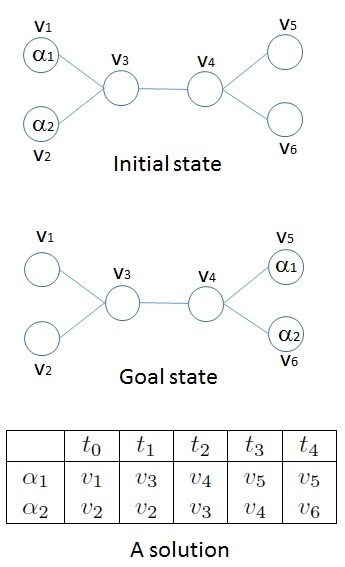
\includegraphics[width=1.5in]{mapf_ex.jpg}
\caption{An instance of the MAPF problem and a solution.}
\label{fig:mapf_ex}
\end{figure}

Figure \ref{fig:mapf_ex} gives a sample instance of the MAPF problem. In the initial state, agent $a_1$ occupies vertex $v_1$, and agent $a_2$ occupies vertex $v_2$. The goal of the problem is to move agent $a_1$  to vertex $v_5$ and agent $a_2$  to vertex $v_6$. Figure \ref{fig:mapf_ex} also shows a solution plan for the problem. At time step $t_0 \rightarrow t_1$, agent $a_1$ moves from vertex $v_1$ to vertex $v_3$, and agent $a_2$ waits at vertex $v_2$. At the next step $t_1 \rightarrow t_2$, agent $a_1$ moves from vertex $v_3$ to vertex $v_4$, and agent $a_2$ moves from vertex $v_2$ to vertex $v_3$. In the solution plan, the end time of agent $a_1$ is 3, the end time of agent $a_2$ is 4, and so the  makespan is 4. %

%\section{The Picat Language and its Constraint Modules}
\section{The Picat Language}
Picat is a logic-based multi-paradigm language that integrates logic programming, functional programming, constraint programming, and scripting. Picat takes many features from other languages, including logic variables, unification, backtracking,  pattern-matching rules, functions, list and array comprehensions, loops, assignments, tabling for dynamic programming and planning, and constraint solving with CP, SAT, and MIP. The reader is referred to \cite{PicatBook15} for the details of the language and the constraint modules.

In Picat, predicates and functions are defined with pattern-matching rules. Picat has two types of rules: the \emph{non-backtrackable} rule: $Head, Cond\ $\verb+=>+$\ Body$ and the \emph{backtrackable} rule: $Head, Cond\ $\verb+?=>+$\ Body$. In a predicate definition, the $Head$ takes the form $p(t_1,\ldots,t_n)$, where $p$ is a predicate name, and $n$ is the arity. The condition $Cond$, which is an optional goal, specifies a condition under which the rule is applicable. For a call $C$, if $C$ matches $Head$ and $Cond$ succeeds, then the rule is said to be \emph{applicable} to $C$. When applying a rule to call $C$, Picat rewrites $C$ into $Body$. If the used rule is backtrackable, then the program will backtrack to $C$ if $Body$ fails.

A \emph{function} is a special kind of a predicate that is defined by non-backtrackable rules. In a function definition, the $Head$ takes the form $f(t_1,\ldots,t_n) = Term$, where $f$ is a function name and $Term$ is a result to be returned. If $Cond$ and $Body$ are both true, then they can be omitted together with the $\verb+=>+$ arrow.

Picat supports \emph{tabling}, which caches previously calculated solutions, and reuses them in subsequent computations. In Picat, both predicates and functions can be tabled.  In order to have all calls and answers of a predicate or function tabled, users just need to add the keyword \texttt{table} before the first rule. For a predicate definition, the keyword \texttt{ table} can be followed by a tuple of table modes, including \texttt{ +} (input), \texttt{ -} (output), \texttt{ min}, \texttt{ max}, and \texttt{ nt} (not tabled). For a predicate with a table mode declaration that contains \texttt{ min} or \texttt{ max}, Picat tables one optimal answer for each tuple of the input arguments. For example, the following predicate \texttt{shortest\_dist}  computes the shortest-path cost of a given pair of vertices in a unit-cost graph that is represented by the predicate \texttt{edge/2}:

\begin{small}
\begin{verbatim}
table (+,min)
shortest_dist((V,V),Cost) => 
    Cost = 0.
shortest_dist((V,FV),Cost) => 
    edge(V,NextV),
    shortest_dist((NextV,FV),Cost1),
    Cost = Cost1+1.
\end{verbatim}
\end{small}

This tabled predicate will be used later to compute lower bounds and preprocessing state variables.\footnote{When applied to finding single-source shortest-path costs, this tabled predicate implements Dijkstra's algorithm, except that it tables shortest-path costs from the encountered vertices to the destination vertex.}

Picat provides three solver modules, \texttt{cp}, \texttt{sat}, and \texttt{mip}, for modeling and solving CSPs. As a constraint programming language, Picat resembles CLP(FD)
%\cite{DIN88}
: the operator \verb+::+ is used for domain constraints, the operators \verb+#=+, \verb+#!=+, \verb+#>+, \verb+#>=+, \verb+#<+, \verb+#<=+, and \verb+#=<+ are used for arithmetic constraints, and the operators \verb+#/\+ (and), \verb+#\/+ (or), \verb+#^+ (xor), \verb+#~+ (not), \verb+#=>+ (if), and \verb+#<=>+ (iff) are used for Boolean constraints. Picat supports several global constraints, such as \texttt{all\_different/1}, \texttt{element/3}, and \texttt{cumulative/4}. In addition to intensional constraints, Picat also supports expressing extensional, or table, constraints. The common interface that Picat provides for the solver modules allows seamless switching from one solver to another, and the basic language constructs, such as arrays, loops, and list comprehensions, make Picat a convenient modeling language for CSPs.

For the \texttt{sat} module, the Picat SAT compiler \cite{ZhouK16,ZhouK17} translates constraints into a logic formula in the conjunctive normal form (CNF) for the underlying SAT solver.  Picat employs the \textit{log-encoding} for compiling domain variables and constraints.  For a domain with the maximum absolute value $n$, $log_2n$ Boolean variables are used. If the domain contains both negative and positive values, then another Boolean variable is used to encode the sign. Each combination of values of these Boolean variables represents a valuation for the domain variable. PicatSAT flattens constraints into primitive ones, and performs numerous optimizations, both in the phase of breaking constraints into primitive ones, and in the phase of compiling primitive constraints into adders and comparators \cite{ZhouK17}. For optimization problems, Picat uses branch-and-bound to optimize the objective. It first posts the problem as a constraint satisfaction problem, ignoring the objective. Once a solution is found, Picat uses binary search to find a solution with the optimum value.

For the {\tt mip} module, constraints are compiled into inequality ($\le$) constraints. The compilation follows the standard textbook recipe \cite{BertsimasW05}. For example, the reification constraint \verb&B #<=> (X #=< Y)& is translated into \verb&X-Y-M1*(1-B) #=< 0& and \verb&Y-X+1-M2*B #=< 0&, where {\tt M1} and {\tt M2} are constants:
\begin{small}
\begin{verbatim}
    M1 = ubd(X)-lbd(Y)+1
    M2 = ubd(Y)-lbd(X)+2
\end{verbatim}
\end{small}
where {\tt ubd(X)} is the upper bound of the domain of {\tt X}, and {\tt lbd(X)} is the lower bound. The compiler avoids introducing big constants when linearizing constraints if possible. For example, the constraint \verb&B #=> (sum(L) #>= C)&, where \texttt{L} is a list of non-negative integer-domain variables and \texttt{C} is a positive constant, is translated into \verb&sum(L) #>= C*B&. 

\section{A MAPF Model and its Implementation in Picat}
This section gives a CSP model for MAPF, together with its implementation in Picat, which optimizes the makespan. This section also gives a technique for preprocessing the state variables, and an extended program for optimizing the sum-of-costs for a given makespan.

\subsection{The MAPF Model}
We can model the MAPF problem as a CSP, following the planning-as-satisfiability framework \cite{KautzS92}. We use a Boolean variable $B_{t a v}$ to indicate if agent $a$ ($a = 1, 2, \ldots, k$) occupies vertex $v$ ($v = 1, 2, \ldots, n$) at time $t$ ($t = 0, 1,\ldots, m$). The following constraints ensure the validity of every state and every transition:
\begin{description}
\item[(1)] Each agent occupies exactly one vertex at each time.
\begin{tabbing}
aa \= aaa \= aaa \= aaa \= aaa \= aaa \= aaa \kill
$\Sigma_{v=1}^{n} B_{t a v} = 1$ for $t = 0, \ldots, m$, and $a = 1, \ldots, k$.  
\end{tabbing}

\item[(2)] No two agents occupy the same vertex at any time.
\begin{tabbing}
aa \= aaa \= aaa \= aaa \= aaa \= aaa \= aaa \kill
$\Sigma_{a=1}^{k} B_{t a v} \le 1$ for $t = 0, \ldots, m$, and $v = 1, \ldots, n$. 
\end{tabbing}

\item[(3)] If agent $a$ occupies vertex $v$ at time $t$, then $a$ occupies a neighboring vertex at time $t+1$. \footnote{Recall that we assume the graph is reflexive.}
\begin{tabbing}
aa \= aaa \= aaa \= aaa \= aaa \= aaa \= aaa \kill
$B_{t a v} = 1 \Rightarrow \Sigma_{u \in neibs(v)}(B_{(t+1) a u}) \ge 1$ \\
for $t = 0, \ldots, m-1$, $a = 1, \ldots, k$, and $v = 1, \ldots, n$.  \\ 
\end{tabbing}
\end{description}
Note that constraints (1) and (3) entail that
\begin{tabbing}
aa \= aaa \= aaa \= aaa \= aaa \= aaa \= aaa \kill
\> $B_{t a v} = 1 \Rightarrow \Sigma_{u \in neibs(v)}(B_{(t+1) a u}) = 1$,
\end{tabbing}
for $t = 0, \ldots, m-1$, $a = 1, \ldots, k$, and $v = 1, \ldots, n$.  It is more efficient to use inequality ($\ge$) in constraint (3) than equality, because the inequality constraint can be compiled into one CNF clause.
%Also note that the additional no-edge-crossing and no-rotating constraints, which were mentioned above, can easily be added into the model. (RB: It was not mentioned in the text so far)

The model consists of $k\times(m+1)\times n$ Boolean variables, where $k$ is the number of agents, $m$ is the makespan, and $n$ is the number of vertices in the graph. The \textit{exactly-one} constraint $\Sigma_{v=1}^{n} B_{t a v} = 1$ in (1) is encoded as a conjunction of the \textit{at-least-one} constraint $\Sigma_{v=1}^{n} B_{t a v} \ge 1$ and the \textit{at-most-one} (AMO) constraint $\Sigma_{v=1}^{n} B_{t a v} \le 1$. The at-least-one constraint is encoded as one clause. The number of clauses generated from the constraints in the model depends on how the AMO constraint is encoded. The PicatSAT compiler employs the \textit{2-product algorithm} \cite{JChen10}, which encodes the summation $\Sigma_{i=1}^{l} B_i$ in the AMO constraint as the Cartesian product of two subsets of Boolean variables. Based on this encoding, the model requires $O(m\times k\times \sqrt{n}+ m\times n \times \sqrt{k})$ auxiliary variables and $O(m\times k \times n)$ clauses to encode.


\begin{figure}[!t]
\begin{small}
\begin{verbatim}
import sat.

path(N,As) =>
    K = len(As),
    lower_upper_bounds(As,LB,UB),
    between(LB,UB,M),
    B = new_array(M+1,K,N),
    B :: 0..1,

    % Initialize the first and last states
    foreach (A in 1..K)    
        (V,FV) = As[A],
        B[1,A,V] = 1,
        B[M+1,A,FV] = 1
    end,

    % Each agent occupies exactly one vertex 
    foreach (T in 1..M+1, A in 1..K)
        sum([B[T,A,V] : V in 1..N]) #= 1
    end,

    % No two agents occupy the same vertex 
    foreach (T in 1..M+1, V in 1..N) 
        sum([B[T,A,V] : A in 1..K]) #=< 1   
    end,

    % Every transition is valid
    foreach (T in 1..M, A in 1..K, V in 1..N) 
        neibs(V,Neibs),
        B[T,A,V] #=> 
        sum([B[T+1,A,U] : U in Neibs]) #>= 1
    end,

    solve(B),
    output_plan(B).
\end{verbatim}
\end{small}
\caption{A program in Picat for MAPF.}
\label{fig:mapf_sat}
\end{figure}

\subsection{The Implementation in Picat}
Figure \ref{fig:mapf_sat} shows an implementation of the CSP  model in Picat. The program uses the \texttt{sat} module. We can switch to \texttt{mip} or \texttt{cp} by changing the import declaration.

For a given MAPF problem, the graph is represented by the predicate \texttt{neibs(V,Neibs)}, which binds \texttt{Neibs} to the list of the neighboring vertices of a given vertex \texttt{V}. Let \texttt{N} be the number of vertices in the graph, and \texttt{As} be a list of agents, where each agent is a pair that indicates the starting and ending vertices of the agent. The predicate \texttt{path(N,As)} finds a path for each of the agents.

The function call \texttt{len(As)} returns the number of agents (the length of the list). The predicate
\begin{verbatim}
  lower_upper_bounds(As,LB,UB)
\end{verbatim}
computes the lower and upper bounds on an optimal makespan. The lower bound, \texttt{LB}, is the maximum of the shortest-path costs, which is the number of steps required to move the most difficult agent from its initial vertex to its destination vertex. The upper bound, \texttt{UB}, is the sum of the shortest-path costs. If only one agent is allowed to move at each step, then \texttt{UB} is the number of steps required to move all of the agents to their destinations.\footnote{Note that it is assumed that there is a path connecting each agent's starting vertex to its destination vertex; otherwise, the predicate \texttt{lower\_upper\_bounds} fails.}

The predicate call \texttt{between(LB,UB,M)} generates a number \texttt{M} between \texttt{LB} and \texttt{UB}; it generates the next number on backtracking. If a plan is found for a value of \texttt{M}, then the plan is guaranteed to be optimal with the makespan \texttt{M}. Otherwise, if no plan is found for the value, then the program backtracks to \texttt{between} to generate the next number. This \textit{generate-and-test} step is repeated until a plan is found for some value \texttt{M}, or until no plan is found after all of the numbers in the range \texttt{LB..UB} have been tried.

The function call \texttt{new\_array(M+1,K,N)} creates a three dimensional array, where the first dimension indicates the time points from 1 through \texttt{M+1}, the second dimension refers to the agents \texttt{1..K}, and the third dimension represents the vertices \texttt{1..N}. The call \texttt{B :: 0..1} changes the entries of the array \texttt{B} to Boolean variables, which are 0/1 integer domain variables.

There are four \texttt{foreach} loops in the encoding. The first \texttt{foreach} loop initializes the first and last states. For an agent \texttt{A} whose initial vertex is \texttt{V} and whose goal vertex is \texttt{FV}, the entries \texttt{B[1,A,V]} and \texttt{B[M+1,A,FV]} are set to 1. Note that, since array indices in Picat are 1-based, the initial state has index 1, and the goal state has index \texttt{M+1}. The remaining three \texttt{foreach} loops encode the constraints (1), (2), and (3) in the model.

The call \texttt{solve(B)} performs three operations: (1) it compiles all the accumulated constraints into CNF; (2) it calls the SAT solver to solve the CNF formula; (3) it retrieves the solution from the SAT solver and produces bindings for the variables in B. If a different solver module is imported, then constraints are translated into different encodings.

\subsection{\label{sec:improv}Preprocessing}
Consider an agent $a$ whose starting vertex is $start(a)$ and whose goal vertex is $goal(a)$. For a vertex $v$, let $d(s,v)$ be the shortest distance from $start(a)$ to $v$, and $d(v,g)$ be the shortest distance from $v$ to $goal(a)$. Agent $a$ cannot occupy vertex $v$ at times $t = 0, 1, \ldots, d(s,v)-1$:
\begin{tabbing}
aa \= aaa \= aaa \= aaa \= aaa \= aaa \= aaa \kill
\> $B_{t a v} = 0$ for $t = 0, 1, \ldots, d(s,v)-1$.
\end{tabbing}
Similarly, agent $a$ cannot occupy vertex $v$ at times $t = m-d(v,g)+1, \ldots, m$:
\begin{tabbing}
aa \= aaa \= aaa \= aaa \= aaa \= aaa \= aaa \kill
\> $B_{t a v} = 0$ for $t = m-d(v,g)+1, \ldots, m$.
\end{tabbing}

The preprocessing phase requires finding shortest-path costs and setting the variables, which takes $O(k\times n^2 + k \times n \times m)$ overall running time, where $k$ is the number of agents, $m$ is the makespan, and $n$ is the number of vertices.  For large graphs, this complexity is prohibitive. For grid maps, Manhattan distances can be substituted as estimates of shortest-path costs.

\section{Modeling MAPF Variants}
\label{sec:modelingMAPFVariants}
The MAPF problem has many variants that correspond to the broad range of MAPF applications. 
One of the main strengths of using constraint programming in general and Picat in particular is the ease with which one can support different variants of the problem. In this section, we demonstrate how important variants of MAPF can be  encoded using our Picat modeling by making only minimal changes to the encoding. 


\subsection{\label{sec:model}The Sum-of-Costs Objective}


The declarative model described above is designed to optimize for makespan. However, different objective functions have been studied for MAPF, such as finding a plan with minimum sum of costs.

\begin{definition}[Sum of costs]
The \textit{sum-of-costs} (SOC) of a plan is the sum of the end times of the paths in the plan. 
\end{definition}
In the MAPF example depicted in Figure~\ref{fig:mapf_ex}, the SOC is 7. 


We can easily extend the core model to make it find a plan with the minimum sum-of-costs instead of minimum makespan. To this end, we introduce a variable $E_a$ for each agent $a$ ($a = 1,2,..., k$) that represents the end time of the agent. The domain of $E_a$ has the cost of the shortest path from $a$'s initial vertex to its goal vertex as its lower bound, and the maximum makespan as its upper bound.

Let $goal(a)$ be $g$, $a$'s goal vertex. The following constraints enforce that the agent reaches its goal at time $E_a$ and stays at the goal afterwards.
\begin{description}
\item[(4)] Agent $a$ reaches its goal vertex $g$ at time $E_a$, i.e., agent $a$ does not occupy vertex $g$ at time $E_a-1$:
\begin{tabbing}
aa \= aaa \= aaa \= aaa \= aaa \= aaa \= aaa \kill
For $t = 2, 3, \ldots, m$, $E_a = t \rightarrow B_{(t-1) a g} = 0$.
\end{tabbing}

\item[(5)] Agent $a$ occupies vertex $g$ from time $E_t$ through  $m$.
\begin{tabbing}
aa \= aaa \= aaa \= aaa \= aaa \= aaa \= aaa \kill
\> For $t = E_a, E_a+1, \ldots, m,\  B_{t a g} = 1$.
\end{tabbing}
\end{description}
The objective is to minimize the sum-of-costs: \texttt{min($\Sigma_{a=1}^kE_a$)}.
\begin{figure}
\begin{small}
\begin{verbatim}
end_time(B,As,K,M,E) =>
    E = new_array(K),
    E :: 1..M+1,
    foreach (A in 1..K, T in 1..M+1)
        (V,FV) = As[A],
        if T > 1 then
            E[A] #= T #=> B[T-1,A,FV] #= 0
        end,
        foreach (T1 in T..M+1)
            E[A] #= T #=> B[T1,A,FV] #= 1
        end
    end.
\end{verbatim}
\end{small}
\caption{The Picat code for constraints (4) and (5) in the sum of costs model.}
\label{fig:soc-encoding}
\end{figure}
The predicate given in Figure~\ref{fig:soc-encoding} encodes constraints (4) and (5).

The constraint \verb+E[A] #= T #=> B[T-1,A,FV] #= 0+ states that if agent \texttt{A}'s end time is \texttt{T}, then agent \texttt{A} does not occupy the goal vertex \texttt{FV} at time \texttt{T-1}. The inner \texttt{foreach} loop enforces that the agent \texttt{A} occupies the goal vertex \texttt{FV} from time \texttt{T} through \texttt{M+1}.

%In order to modify the program in Figure \ref{fig:mapf_sat} to make it minimize the sum-of-costs for the minimum makespan, we add the call \texttt{end\_time(B,As,K,M,E)} before the call to \texttt{solve}, and change \texttt{solve(B)} to \texttt{solve([\$min(sum(E))],B)},\footnote{The preceding dollar symbol indicates that \texttt{min(sum(E))} is a term, not a function call.} which passes the objective \texttt{min(sum(E))} to the solver.

A straightforward approach to modify the program in Figure \ref{fig:mapf_sat} to make it minimize the overall sum-of-costs is changing the nondeterministic call \texttt{between(LB,UB,M)} to \texttt{M = UB}, adding the call \texttt{end\_time(B,As,K,M,E)} before the call to \texttt{solve}, and changing \texttt{solve(B)} to \texttt{solve([\$min(sum(E))],B)},\footnote{The preceding dollar symbol indicates that \texttt{min(sum(E))} is a term, not a function call.} which passes the objective \texttt{min(sum(E))} to the solver. In this way, the plan found will have the minimum SOC for all possible makespans. This naive approach requires many variables in the model if the upper bound for makespan is large. A more advanced  approach was proposed in \cite{SurynekFSB16} that is based on idea of increasing the makespan together with increasing the limit for the cost function. This reduces the size of the model (the number of variables), but increases the number of calls to the solver (the solver is invoked for every makespan tried).


One can also devise a hybrid objective function: minimizing makespan as a primary objective and minimizing SOC as a secondary objective, i.e., among plans with the same makespan prefer the plan that has the smallest SOC. In order to modify the program in Figure \ref{fig:mapf_sat} to perform this two-stage optimization, we just need to make the same changes as above for optimizing overall SOC, but leaving \texttt{between(LB,UB,M)} as it is.

\subsection{\label{sec:prior}Priorities}
The sum of costs objective assumes that the cost of moving each agent is equal. In many scenarios, however, moving different agents may incur different costs. For example, consider a MAPF problem where all agents represent taxis moving people in a city except for one agent that represents an ambulance driving to the hospital. Clearly, it is more important to minimize the time it takes the ambulance to reach the hospital than to minimize the time spent by the other taxi agents. We can represent such scenarios in a general way by assuming a given vector of weights $\textbf{w}=(w_1,\ldots,w_k)$, 
where $w_i$ is the cost of having agent $a_i$ spend one time step, 
and the corresponding objective function is the {\em weighted sum-of-costs}. 

Adjusting the sum of costs model to support priorities in such a ways is trivial. 
We define a variable $WE = \textbf{w}\cdot E$, which holds the weighted cost of each agent, and pass to the solver the objective \texttt{min(sum(WE))} instead of 
\texttt{min(sum(E))}.

\subsection{Robust Plans}
Since agents may get delayed unexpectedly, 
it is sometimes desirable to create solutions to MAPF problems
that are robust to such changes. One can imagine several forms of such robust planning. 
$L$-robustness is one form of robustness that has been suggested studied in the context of MAPF~\cite{atzmon2017kRobust}. A $L$-robust solution to a MAPF problem is a problem 
that minimizes some objective function (e.g., sum of costs or makespan)
while ensuring that the solution can be executed as long
as there is no agent that will experience more than $L$ unexpected delays. 

\begin{figure}
\small
\centering
\begin{verbatim}
	foreach(T in 1..M1, A in 1..K, V in 1..N)
   		B[T,A,V] #=> sum([B[Prev,A2,V] : 
               A2 in 1..K, A2!=A, 
               Prev in max(1,T-L)..T]) #= 0
	end
\end{verbatim}
\caption{The constraint needed to support finding a $L$-robust solution}
\label{fig:addRobustness}
\end{figure}

Adjusting the Picat model to return $L$-robust solutions is also very simple. 
It involves modifying a constraint that forbids two agents from occupying the same vertex at the same time, such that the constraint forbids every two agents 
from occupying the same vertex in times that are no more than $L$ time steps from each other. Fig.~\ref{fig:addRobustness} shows the exact Picat code for this constraint.
We implemented this variant and observed that in some settings it is comparable to a CBS-based $k$-robust solver~\cite{atzmon2017kRobust}. 


\subsection{Edge Conflicts and Train-like Motion}
Some variants of the problem impose additional constraints on valid paths. 
One constraint requires that when an agent moves from vertex $u$ to $v$ ($u \neq v$) at time $t$, $v$ cannot be occupied by another agent at time $t$. Without this constraint agents can move in a train-like formation, while having this constraint bans such a motion and bans agents from making cyclic rotations in an empty-space-free area \cite{YuL13}. 
Encoding this constraint on top of the Picat model is very easy. In fact, it is equivalent to searching for a 1-robust solution. 

Another constraint that have been used in prior works is to mandate that no two agents can cross each other on an edge at any time step. Under this constraint, when an agent moves from vertex $u$ to vertex $v$ at time step $t \rightarrow (t+1)$, no agent can move from vertex $v$ to vertex $u$ at the same time step. This is known as the {\em edge conflict} constraint. 
Adjusting the model to avoid edge conflicts can be done by adding an explicit constraint that checks for every two agents, every location, and every pair of consecutive time steps that these agents did not swap locations. 
We implemented this extension and observed that it causes substantial increase in runtime, as this constraint translates to many constraints to the underlying solver. 
An alternative implementation can be to maintain a variable for each edge, time step, and agent, to keep track of which edges are being used by the agents. 


Note that we do not claim that all the above is the best encoding
for these variants. More sophisticated encodings might yield shorter runtimes. However, the above encodings are sound 
and easily implemented.


\section{Experimental Results}
This section gives experimental results
comparing a range of solvers, encodings, and MAPF variants. 
We used a random-instance generator that is similar to the one used in \cite{Surynek14} for generating grid maps. 
Of the set of problems we have generated, we chose a set of 20 representative instances under different settings. 
Each instance name takes the form \texttt{gN\_pP\_aK}, where \texttt{N}$\times$\texttt{N} is the grid size, \texttt{P} is the percentage of obstacles, or blocked squares, in the grid, and \texttt{K} is the number of agents. For example, the instance named ``g32\_p20\_a40'' represents a MAPF problem with 40 agents 
on a 32x32 grid 
where 20\% of the grid cells are obstacles. 
Unless stated otherwise, all experiments were run on Cygwin notebook computer with 2.60GHz Intel i7 and 64GB RAM,
and we measured CPU time, in seconds. A time limit was set to 600 seconds.


% In the first set of experiments, we compared different underlying solvers and encodings created all through modifications to our declarative Picat-based model. In the second set of experiments we compared with other state-of-the-art  MAPF declarative models. 
%obtained with three solvers, namely, SAT, MIP, and ASP. In addition to these three solvers, we also experimented with a CP model and a planner model, both in Picat version 2.1. The CP model uses a domain variable for each agent and each time, which indicates the vertex that the agent occupies at the time. The planner model searches the state space using tabled backtracking search. This section will not give results from these solvers, because they are not competitive on large instances.

%Table \ref{tab:res} compares the performances of the three solvers on 20 randomly generated instances under different settings.  The CPU time, in seconds, was obtained on a Cygwin notebook computer with 2.60GHz Intel i7 and 64GB RAM. The time limit was set to 600 seconds. For SAT and MIP, the program presented above for minimizing makespan was used; SAT$_{nop}$ and MIP$_{nop}$ do not perform preprocessing, while SAT$_p$ and MIP$_p$ perform preprocessing. For SAT, the generated CNF code was solved with Lingeling (version 587f) \cite{lingeling}.  For MIP, the generated code was solved with Gurobi version 6.5.1 \cite{gurobi}.  For ASP, the program given in \cite{ErdemKOS13}, which encodes the same constraints and the makespan objective, was run with clingo 4.5.4 \cite{clingon}. For all of the solvers, the CPU time includes both the compilation time (the grounding time for ASP) and the solving time.

Table \ref{tab:res} compares the performances of our declarative model using different underlying solvers, namely SAT and MIP, for finding makespan-optimal plans. We also experimented with a CP model and a planner model, both available in Picat version 2.1. The CP model uses a domain variable for each agent and each time, which indicates the vertex that the agent occupies at the time. The planner model searches the state space using tabled backtracking search. The results of the CP and planner models were very poor on large instances so we do not present their results in this section. 
%This section will not give results from these solvers, because they are not competitive on large instances.
%the three solvers on 20 randomly generated instances under different settings.  The CPU time, in seconds, was obtained on a Cygwin notebook computer with 2.60GHz Intel i7 and 64GB RAM. The time limit was set to 600 seconds. 
For SAT and MIP, we compared the program presented in Figure~\ref{fig:mapf_sat} with the preprocessing described in Section~\ref{sec:improv}, denoted SAT$_p$ and MIP$_p$, and without it, denoted 
SAT$_{nop}$ and MIP$_{nop}$. 
%and without the preprocessing described in Section~\ref{sec:improv}, denoted SAT$_{nop}$ and MIP$_{nop}$ do not perform preprocessing, while SAT$_p$ and MIP$_p$ perform preprocessing. 
For SAT, the generated CNF code was solved with Lingeling (version 587f) \cite{lingeling}.  For MIP, the generated code was solved with Gurobi version 6.5.1 \cite{gurobi}. The best performing algorithm for each instances is highlighted in bold. 

%We used a random-instance generator that is similar to the one used in \cite{Surynek14} for generating grid maps. More instances were tested, and the results given in Table \ref{tab:res} are representative. Each instance name takes the form \texttt{gN\_pP\_aK}, where \texttt{N}$\times$\texttt{N} is the grid size, \texttt{P} is the percentage of obstacles, or blocked squares, in the grid, and \texttt{K} is the number of agents. The number in parentheses following each instance name is the minimum makespan.  All grids are 4-connected, meaning that no diagonal moves are allowed.  All of the instances and the programs used in the experiment are available in the supplementary attachment.


\begin{table}[t]
\caption{\label{tab:res}A comparison of solvers' performance for minimizing makespan (CPU time, seconds)}
\centering
%\begin{scriptsize}
\begin{tabular}{|c|r|r|r|r|}  \cline{1-5}
Instance (M) & SAT$_{nop}$ & SAT$_p$ & MIP$_{nop}$ & MIP$_p$  \\ \hline \hline
%\cline{1-6}\cline{1-6}
g16\_p10\_a05 (14)  & 0.59 &   {\bf 0.27}  & 1.51 & 0.43  \\ \hline
g16\_p10\_a10 (20)  & 2.29 & 1.37 & 4.96 &   {\bf 0.88}   \\ \hline
g16\_p10\_a20 (23)  & 5.73 & 2.76 & 13.14 &   {\bf 2.54}   \\ \hline
g16\_p10\_a30 (23)  & 8.89 &   {\bf 3.11}  & 19.88 & 3.5  \\ \hline
g16\_p10\_a40 (30)  & 24.4 &   {\bf 8.25}  & 119.07 & 72.93  \\ \hline
g16\_p20\_a05 (24)  & 1.7 & 1.01 & 3.23 &   {\bf 0.83}   \\ \hline
g16\_p20\_a10 (24)  & 2.29 &   {\bf 1.50}  & 5.86 & 1.81  \\ \hline
g16\_p20\_a20 (23)  & 4.56 &   {\bf 2.12}  & 11.26 & 2.5  \\ \hline
g16\_p20\_a30 (28)  & 11.63 &   {\bf 4.37}  & 38.31 & 7.06  \\ \hline
g16\_p20\_a40 (22)  & 12.19 &   {\bf 3.48}  & 31.35 & 10.24  \\ \hline
g32\_p10\_a05 (37)  & 7.45 &   {\bf 1.98}  & 24.86 & 2.14  \\ \hline
g32\_p10\_a10 (34)  & 13.63 &   {\bf 3.08}  & 49.74 & 4.15  \\ \hline
g32\_p10\_a20 (42)  & 40.67 &   {\bf 8.71}  & 219.65 & 14.05  \\ \hline
g32\_p10\_a30 (55)  & 82.02 &  {\bf 34.48}  & 380.28 & 167.94  \\ \hline
g32\_p10\_a40 (47)  & 79.49 &  {\bf 34.95}  &  $>$600  & 150.59  \\ \hline
g32\_p20\_a05 (53)  & 11.1 &   {\bf 5.75}  & 54.97 & 9.86  \\ \hline
g32\_p20\_a10 (36)  & 14.03 &   {\bf 2.97}  & 50.56 & 4.99  \\ \hline
g32\_p20\_a20 (49)  & 42.8 &  {\bf 16.93}  & 266.25 & 24.69  \\ \hline
g32\_p20\_a30 (43)  & 53.3 &  {\bf 12.98}  & 248.05 & 43.38  \\ \hline
g32\_p20\_a40 (42)  & 86.66 &  {\bf 16.51}  & 351.55 & 30.89  \\ \hline \hline
Total solved  &  {\bf 20}  &  {\bf 20}  & 19 &  {\bf 20} \\ \hline
\end{tabular}
%\end{scriptsize}
\end{table}


The SAT solver is a clear winner among the two solvers; it easily solved all of the instances within the time limit. For SAT, running time increases with the increase of the number of agents, but the rate is much smaller than that for MIP. Further testing showed that the SAT program successfully solved all of the instances with 100 agents generated for the grid size of $32\times 32$ within the time limit. For the grid size of $32\times 32$, the time taken by the solvers generally decreases when the percentage of obstacles increases from 10\% to 20\%. The increase of obstacles reduces the graph size, and ultimately leads to the decrease of the number of variables in the models. The preprocessing technique is effective for improving the speed of both the SAT and MIP solutions.

The MIP solver is slower than the SAT solver for all of the instances, except for three cases, and its time visibly increases with the increase of the number of agents. Modern MIP solvers adopt some effective solving techniques from SAT solvers. It's unclear whether Gurobi uses SAT solving techniques or the traditional relaxation method for the generated MIP code.



\begin{table*}[t]
\caption{\label{tab:ressoc}A comparison of solvers' performance for minimizing sum-of-costs (CPU time, seconds)}
\centering
%\begin{scriptsize}
  \begin{tabular}{|c||r|r||r|r|r|r||r|r|r|r|}  \cline{1-11}
\multirow{2}{*}{Instance (SOC)} & \multicolumn{2}{ |c|| }{makespan+SOC} & \multicolumn{4}{ |c|| }{SOC} & \multicolumn{4}{ |c| }{SOC with priorities}\\ \cline{2-11}

& SAT & MIP & SAT$_{naive}$ & SAT$_{adv}$ & MIP$_{naive}$ & MIP$_{adv}$& SAT$_{naive}$ & SAT$_{adv}$ & MIP$_{naive}$ & MIP$_{adv}$ \\ \hline \hline
%\cline{1-11} \cline{1-11}
g16\_p10\_a05 (55) &  0.85 &  {\bf 0.35} & 19.70 & 5.68 & 8.07 & {\bf 2.46} & 24.45 & 64.57 & {\bf 10.85} & 71.67 \\ \hline
g16\_p10\_a10 (126) &  8.48 &  {\bf 1.10} & 64.80 & 35.82 & 69.38 & {\bf 24.49} & 127.67 & $>$600 & {\bf 96.50} & $>$600 \\ \hline
g16\_p10\_a20 (240) & 21.60 &  {\bf 3.05} & 453.06 & {\bf 143.35} & 82.38 & 336.93 & $>$600 & $>$600 & $>$600 & $>$600 \\ \hline
g16\_p10\_a30 (376) & {\bf 23.38} & $>$600 & $>$600 & {\bf 495.04} & $>$600 & $>$600 & $>$600 & $>$600 & $>$600 & $>$600 \\ \hline
g16\_p10\_a40 (526) & {\bf 97.03} & $>$600 & $>$600 & $>$600 & $>$600 & $>$600 & $>$600 & $>$600 & $>$600 & $>$600 \\ \hline
g16\_p20\_a05 (66) &  3.84 &  {\bf 0.97} & 26.16 & 16.20 & 10.76 & {\bf 8.14} & 33.64 & 90.28 & {\bf 14.04} & 109.80 \\ \hline
g16\_p20\_a10 (141) & 11.62 &  {\bf 2.70} & 96.74 & {\bf 92.16} & 224.21 & 153.02 & {\bf 121.09} & $>$600 & 231.45 & $>$600 \\ \hline
g16\_p20\_a20 (278) & {\bf 16.91} & 17.66 & 528.72 & {\bf 209.74} & $>$600 & $>$600 & $>$600 & $>$600 & $>$600 & $>$600 \\ \hline
g16\_p20\_a30 (423) & {\bf 60.02} & $>$600 & $>$600 & $>$600 & $>$600 & $>$600 & $>$600 & $>$600 & $>$600 & $>$600 \\ \hline
g16\_p20\_a40 (520) & {\bf 46.87} & $>$600 & $>$600 & $>$600 & $>$600 & $>$600 & $>$600 & $>$600 & $>$600 & $>$600 \\ \hline
g32\_p10\_a05 (124) & 14.70 &  {\bf 2.65} & 230.50 & {\bf 29.91} & 93.46 & 42.08 & 264.88 & $>$600 & {\bf 115.94} & $>$600 \\ \hline
g32\_p10\_a10 (218) & {\bf 18.99} & 34.95 & $>$600 & {\bf 84.92} & $>$600 & 176.39 & $>$600 & $>$600 & $>$600 & $>$600 \\ \hline
g32\_p10\_a20 (446) & 76.22 & {\bf 18.53} & $>$600 & {\bf 586.71} & $>$600 & $>$600 & $>$600 & $>$600 & $>$600 & $>$600 \\ \hline
g32\_p10\_a30 (738) & {\bf 421.21} & $>$600 & $>$600 & $>$600 & $>$600 & $>$600 & $>$600 & $>$600 & $>$600 & $>$600 \\ \hline
g32\_p10\_a40 (960) & {\bf 361.32} & $>$600 & $>$600 & $>$600 & $>$600 & $>$600 & $>$600 & $>$600 & $>$600 & $>$600\\ \hline
g32\_p20\_a05 (125) & 41.26 & {\bf 13.55} & 181.86 & {\bf 58.27} & 131.99 & 196.74 & 260.22 & $>$600 & {\bf 151.30} & $>$600 \\ \hline
g32\_p20\_a10 (253) & {\bf 25.44} & 66.38 & $>$600 & {\bf 112.20} & $>$600 & $>$600 & $>$600 & $>$600 & $>$600 & $>$600\\ \hline
g32\_p20\_a20 (481) & {\bf 195.75} & $>$600 & $>$600 & $>$600 & $>$600 & $>$600 & $>$600 & $>$600 & $>$600 & $>$600 \\ \hline
g32\_p20\_a30 (852) & {\bf 123.50} & $>$600 & $>$600 & $>$600 & $>$600 & $>$600 & $>$600 & $>$600 & $>$600 & $>$600 \\ \hline
g32\_p20\_a40 (1050) & {\bf 197.33} & $>$600 & $>$600 & $>$600 & $>$600 & $>$600 & $>$600 & $>$600 & $>$600 & $>$600 \\ \hline \hline
Total solved & {\bf 20} & 11 & 8 & {\bf 12} & 7 & 8 & {\bf 6} & 2 & {\bf 6} & 2 \\ \hline
\end{tabular}
%\end{scriptsize}
\end{table*}

Table \ref{tab:ressoc} gives the CPU time taken to find a plan with the minimum sum-of-costs (SOC). We present the results to find a plan with the minimum SOC among those with the shortest makespan (columns makespan+SOC), to find a plan with the overall minimum SOC (columns SOC), and to find a plan with the overall minimum weighted SOC (columns SOC with priorities, see Section~\ref{sec:prior}). Although makespan and sum-of-costs are two objectives that cannot generally be simultaneously optimized, for the instances in Table 2, plans with the minimum sum-of-costs happen to have the shortest makespans too. In the case makespan+SOC, SAT solved all the instances, while MIP failed to solve nine of the instances within the time limit. There  is a perception that MIP is more suited to arithmetic constraints than SAT. This experiment shows that log-encoded SAT code \cite{ZhouK17} is competitive for the model, despite that the objective function involves multiple integer-domain variables. The model for optimizing the overall minimum sum-of-costs is significantly slower than the model that minimizes makespan before minimizing sum-of-costs. We present the results for the straightforward approach (the makespan is set to its upper bound) and a more advanced approach, where the makespan increases synchronously with the bound for SOC \cite{SurynekFSB16}. This advanced approach is clearly more efficient though still behind optimizing makespan first. Finally, after adding priorities to agents, we increased the role of numerical objective and the MIP solver was the best there. Notice also that the straightforward model is better in this setting as it requires a single call to the solver, while the advanced model tries many makespans. This indicates that there is an interesting relation between the satisfiability component (path finding, no-conflict constraints) and numerical objective.


\begin{table}[t]
\caption{\label{tab:resglob}A comparison with the state-of-the-art  (CPU time, seconds)}
\centering
%\begin{scriptsize}
  \begin{tabular}{|c||r|r|r||r|r|r|}  \cline{1-7}
\multirow{2}{*}{Instance} & \multicolumn{3}{ |c|| }{Makespan} & \multicolumn{3}{ |c| }{Sum of costs} \\ \cline{2-7}

              & Picat & MDD & ASP & Picat & MDD & ICBS \\ \hline \hline
% \cline{1-7}\cline{1-7}
g16\_p10\_a05  & 0.27 & 0.02 & 10.86 & 5.68 & 0.01 & 0.01\\ \hline
g16\_p10\_a10  & 1.37 & 0.14 & 9.58 & 35.82 & 0.01 & 0.01\\ \hline
g16\_p10\_a20  & 2.76 & 0.76 & 26.06 & 143.35 & 0.01&  0.01\\ \hline
g16\_p10\_a30  & 3.11 & 0.79 &  $>$600   & 495.04 & 0.52&  0.02\\ \hline
g16\_p10\_a40  & 8.25 & 4.71 &  $>$600   &  $>$600  & 107.95&  $>$600\\ \hline
g16\_p20\_a05  & 1.01 & 0.16 & 5.96 & 16.2 & 0.01 & 0.01\\ \hline
g16\_p20\_a10  & 1.5 & 0.31 & 18.59 & 92.16 & 1.58 & 0.16\\ \hline
g16\_p20\_a20  & 2.12 & 0.46 & 20.71 & 209.74 & 0.6 & 0.05\\ \hline
g16\_p20\_a30  & 4.37 & 1.45 &  $>$600   &  $>$600  &  $>$600 &  $>$600\\ \hline
g16\_p20\_a40  & 3.48 & 1.15 &  $>$600   &  $>$600  &  $>$600 &  $>$600\\ \hline
g32\_p10\_a05  & 1.98 & 0.53 & 12.93 & 29.91 & 0.01 & 0.01\\ \hline
g32\_p10\_a10  & 3.08 & 1.21 & 31.34 & 84.92 & 0.01 & 0.01\\ \hline
g32\_p10\_a20  & 8.71 & 6.8 & 105.47 & 586.71 & 0.03 & 0.01\\ \hline
g32\_p10\_a30  & 34.48 & 40.13 & 274.11 &  $>$600  & 0.22 & 0.02\\ \hline
g32\_p10\_a40  & 34.95 & 24.87 &  $>$600   &  $>$600  & 1.81 & 0.34\\ \hline
g32\_p20\_a05  & 5.75 & 2.77 & 11.99 & 58.27 & 0.01 &  0.01 \\ \hline
g32\_p20\_a10  & 2.97 & 1.11 & 33.22 & 112.2 & 0.09 &  0.01 \\ \hline
g32\_p20\_a20  & 16.93 & 13.73 & 101.84 &  $>$600  & 2.5&  0.22\\ \hline
g32\_p20\_a30  & 12.98 & 4.54 & 199.69 &  $>$600  & 1.78 & 0.05\\ \hline
g32\_p20\_a40  & 16.51 & 8.17 & 418.56 &  $>$600  & 3.24 & 0.13\\ \hline \hline

Total solved  & 20 & 20 & 15 & 12 & 18 & 17  \\ \hline
\end{tabular}
%\end{scriptsize}
\end{table}

Table~\ref{tab:resglob} compares the performance of our best model -- using a compilation to SAT and with the aforementioned preprocessing  -- with other state-of-the-art declarative models based on SAT and ASP. 
For ASP, the program given in \cite{ErdemKOS13}, which encodes the same constraints and the makespan objective, was run with {\tt clingo 4.5.4} \cite{clingon}. For SAT, we used MDD-SAT, which uses an encoding very similar to ours. MDD-SAT uses a similar  preprocessing as we do based on reachability of vertices w.r.t. to distance from starting position and goal at given time-step. In addition, MDD-SAT reduces significantly the number of variables and constraints needed to encode bounds of the sum-of-costs by considering only those movements of agents that contribute to the cost above the sum individual costs (sum of lengths of shortest paths connecting start and goal per individual agents).
% Pavel finish edit

For all of the solvers, the CPU time include both the compilation time (the grounding time for ASP) and the solving time. 
Note that there is no available ASP solver for minimizing SOC. 
The results show that the ASP solver is clearly the slowest.  It is very sensitive to the increase of the number of agents. {\tt Clingo} succeeded in finding at least one plan for each of the instances, but failed to find optimal plans for 5 of the instances within the time limit. These results are consistent with the ones reported in \cite{ErdemKOS13}. 
The performance of our model and MDD-SAT is very similar for makespan. For the at-most-one constraint, which is intensively used, MDD-SAT uses the sequential counter encoding \cite{Sinz05} while Picat uses the product encoding \cite{JChen10}. For sum-of-costs, there is a clear advantage to MDD-SAT. We conjecture that this is due to a more advanced form of pre-processing employed in MDD-SAT, which uses the full shortest path to prune variables instead of the Manhattan distance,  
%[[Roni: I wrote my hypothesis for now as a place holder, the previous sentence may be changed later when we have a better understanding of what's going on ]]
% Pavel start edit
%[[Pavel:true reason is propagation of cost bound]]
and also due to encoding of the sum-of-costs bound based on sequential counter that enables efficient Boolean constraint propagation within the SAT solver. 

% Pavel finish edit (Roni made some changes, I hope it is Ok)
The main contribution of this work is not in new state-of-the-art results for all MAPF variants, but in a declarative model that is easily adaptable to different objectives and variables. For example, there is no ASP or sophisticated SAT-based solutions for supporting different agent priorities. As shown in Section~\ref{sec:modelingMAPFVariants} and empirically in Table~\ref{tab:ressoc}, we can support such variants as well as others easily with our Picat model. 



\section{Related Work and Discussion}
The literature in MAPF is abundant. A mini-survey of both algorithmic and declarative solutions to MAPF can be found in \cite{SharonSGF13}. In this section, we only discuss related declarative models for MAPF.
Our CSP model follows the planning-as-satisfiability framework \cite{HuangCZ10,KautzS92,Rintanen12}. Declarative models that are based on the same framework have been proposed for SAT \cite{Surynek14}, ASP \cite{ErdemKOS13}, and CP \cite{Ryan10} solvers. The ASP encoding is arguably the most concise and elegant one. As we showed experimentally, our model is more efficient. More importantly, the downside of ASP is its lack of flexibility in expressing low-level constraints and control knowledge. For example, in ASP, it is difficult to implement the use of greater-than rather than equality in the transition constraint $B_{t a v} = 1 \Rightarrow \Sigma_{u \in neibs(v)}(B_{(t+1) a u}) \ge 1$, the preprocessing technique for eliminating variables, and the generate-and-test algorithm utilized to optimize makespan.
% [[Roni: I removed both paragraphs as now we have an empirical comparison]] Our model for optimizing the makespan objective bears close resemblance to Surynek's model proposed for SAT \cite{Surynek14}. The key constraint used in the model is the at-most-one (AMO) constraint. The PicatSAT compiler uses Chen's algorithm \cite{JChen10}, which encodes a vector of Boolean variables as the product of two smaller vectors of Boolean variables, while Surynek's model uses a naive algorithm, which splits the AMO constraint into smaller AMO constraints on all pairs of variables. Chen's algorithm has better scalability than the naive algorithm for large graphs.
% Our encoding of the sum-of-costs objective is based on the SAT-based encoding proposed in \cite{SurynekFSB16}. There are, however, some differences between these encodings. In our encoding, an integer-domain variable is used to represent the end-time of each agent, and the objective is the sum of all of the end-time variables. The PicatSAT compiler \cite{ZhouK16,ZhouK17} splits the objective expression into triplets, and encodes triplets as optimized logical adders. This encoding is compact, but requires $log_2k$ time to propagate changes from individual variables to the sum variable, where $k$ is the number of end-time variables. As shown in the 2016 MiniZinc Challenge results,\footnote{\url{http://www.minizinc.org/}} the optimized log-encoding that is adopted in PicatSAT is very competitive. %The program proposed in \cite{SurynekFSB16} relies on the cardinality  constraint \cite{Sinz05}, the MDD encoding algorithm \cite{SrinivasanKMB90}, and heuristics to optimize the sum-of-costs. [[Roni all this is not clear: we use the same MDD trick in the pre-process. Which heuristics are you referring to?]]
The preprocessing technique for eliminating variables is well-used in constraint programming for maintaining consistency of some of the global constraints, such as the \textit{regular} constraint \cite{Pesant04}. %This technique is effective for pathfinding: if it is known that a state variable cannot have a value at a certain time, then the value can be excluded from the domain of the variable.[[Roni: why is this relevant here?]]

\ignore{
  In \cite{YuL15d}, a declarative model that formulates MAPF as a network flow problem is given. Experimental results are reported for optimizing four different types of objectives. While a direct comparison is impossible at this stage, an indirect comparison also reveals the competitiveness of our solution. In \cite{YuL15d}, heuristics that do not preserve optimality of plans are used in order to solve instances for the grid size of $32\times 32$.
}

\section{Conclusion}
We have presented a constraint-based declarative model and its implementation in Picat using SAT and MIP for the MAPF problem. The model is easy, and the implementation is concise. Declarative solutions tend to suffer from poor performance. Nevertheless, we have shown that our declarative solution using SAT is more competitive than existing declarative solutions. Our solution can easily be altered for other variants and objectives. Further work includes comparison with other solvers on more benchmarks and exploitation of domain knowledge, such as graph structures, for better performance.

\ignore{
\section*{Acknowledgements}
The authors would like to thank Esra Erdem for giving advice on running the ASP program, Pavel Surynek for providing MDD-SAT and clarifying differences in encodings, and Jonathan Fruhman for valuable comments on the presentation. Neng-Fa Zhou is supported in part by the NSF under grant number CCF1618046, and Roman Bart\'{a}k is supported the Czech Science Foundation under the project P202/12/G061 and together with Roni Stern by the Czech-Israeli Cooperative Scientific Research Project 8G15027.
}
\bibliographystyle{plain}
\bibliography{bibliography-file}
\end{document}


